
\documentclass[journal]{IEEEtran}
\usepackage{tikz}
\usetikzlibrary{arrows,positioning}
\usetikzlibrary{arrows.meta}

\begin{document}


\begin{figure}
\begin{center}
\begin{tikzpicture}
\useasboundingbox[red] (-0.25, -0.5) rectangle (8.25, 2);
\node (omlabel1) at (3.5, 1) {$t$};
\draw[-{Latex[length=2mm]}] (0, 1) -- (omlabel1);
\draw[-{Latex[length=2mm]}] (0, 1) -- (0, 2);
\node[anchor=south west,inner sep=0] at (0, 0) {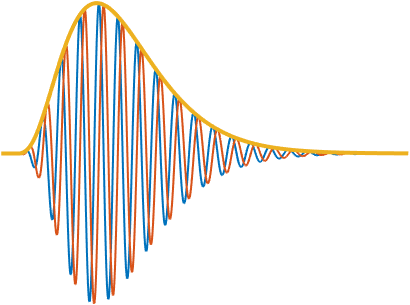
\includegraphics[height=2cm,width=3cm]{gammatone_Q8.png}};
\node at (2, -0.25) {(a)};
\node (omlabel2) at (8, 1) {$t$};
\draw[-{Latex[length=2mm]}] (4.5, 1) -- (omlabel2);
\draw[-{Latex[length=2mm]}] (4.5, 1) -- (4.5, 2);
\node[anchor=south west,inner sep=0] at (4.5, 0) {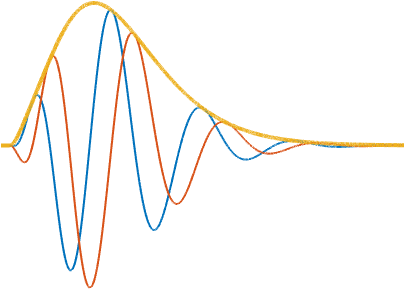
\includegraphics[height=2cm,width=3cm]{gammatone_Q1.png}};
\node at (6.5, -0.25) {(b)};
\end{tikzpicture}
\caption{
\label{fig:gammatones}
Gammatone wavelets $\psi(t)$ in the time domain with quality factors (a) $Q = 4$ and (b) $Q = 1$. Blue and red oscillations represent the real and imaginary parts. The orange envelope represents the complex modulus.}
\end{center}
\end{figure}

\end{document}